\documentclass[12pt]{article}
\usepackage{amsmath,amssymb,amsthm}
\usepackage{graphicx,mathabx}
\usepackage{xcolor}
\usepackage{tikz}
\usepackage{placeins}
\usepackage{lipsum}
\usepackage[shortlabels]{enumitem}
\begin{document}
\title{TCSS 343 - Week 1}
\author{Jake McKenzie}
\maketitle
\noindent\centerline{\textbf{Asymptotics}}\\\\
Exact answers are nice when you can find them. Often times we can't or don't care to find them. As computer scientists we care about the behaivor of the algorithms we employ. If we run into a recurrence relation or summation that expressed loosly the behaivor of these algorithms we'd like to know something about their runtime.\\\\
\centerline{\textbf{Asymptotic Notation in Seven Words}}\\
\centerline{\textbf{suppress constant factors and lower-order terms}}\\\\
Constant factors are things that will be language and system dependent while lower order terms are irrelevant for large inputs.\\\\
Now consider these definitions:\\
\textbf{Big-O Notation}\\
If $\lim\limits_{n\to\infty}{\frac{f(n)}{g(n)}}\to0$ then $f(n) \in O(g(n))$\\\\
This is another way of saying that $f(n) \leq c \cdot g(n)$ for some position $c$.\\
\textbf{Big-$\Omega$ Notation}\\
If $\lim\limits_{n\to\infty}{\frac{f(n)}{g(n)}}\to\infty$ then $f(n) \in \Omega(g(n))$\\\\
This is another way of saying that $f(n) \geq c \cdot g(n)$ for some position $c$.\\
\textbf{Big-$\Theta$ Notation}\\
If $\lim\limits_{n\to\infty}{\frac{f(n)}{g(n)}}\to k$ where k is a positive finite number then $f(n) \in \Theta(g(n))$\\\\
This is another way of saying that $f(n) \in O(g(n))$ and $f(n) \in \Theta(g(n))$\.\\
Now while we're in this course, we will typically need to show that these relationships are true when prompted, but it's always good to know that the following is true where \begin{math}0 < \epsilon < 1 < c\end{math}.\\
\[1 < \log{\log{n}} < \log{n} < n^{\epsilon} < n^c < n^{log{n}} < c^n < n^n < c^{c^{n}}\]\\
This asymptotic pecking order above is from Don Knuth's Concrete Mathematics.\\\\
Now consider the following truths I found in Tim Roughgarden's Algorithms Illuminated: \\
$$\max\{f(n),g(n)\} \leq f(n) + g(n) \land  2 \cdot \max\{f(n),g(n)\} \geq f(n) + g(n)$$
(reminder that $\land$ is the logical ``and" symbol.)\\\\
1. Prove the following  by using the definitions that I've given prior and the information immediately above to show that $\max\{f(n),g(n)\}\in\Theta(f(n) + g(n))$
\newpage
\noindent 2. Arrange the following functions in order of increasing growth rate, with $g(n)$ following $f(n)$ in your list if and only if $f(n) \in O(g(n))$. That means using the limit definitions I gave you or by induction. You cannot simply use Don's asymptotic pecking order I stated but I strongly suggest you use the asymptotic pecking order as a guide to the neighborhood of a correct answer.\\
\begin{enumerate}[a)]
\item $\sum\limits_{i = 0}^{n} 2^i$\\
\item $n^2$\\
\item $n^{0.9999999}\log{n}$\\
\item $1.00001^n$\\
\item $\log{2^{\frac{n}{2}}}$\\
\item $1000000n$\\
\end{enumerate}
\newpage
\noindent 3. Arrange the following functions in order of increasing growth rate, with $g(n)$ following $f(n)$ in your list if and only if $f(n) \in O(g(n))$. That means using the limit definitions I gave you or by induction. You cannot simply use Don's asymptotic pecking order I stated but I strongly suggest you use the asymptotic pecking order as a guide to the neighborhood of a correct answer.\\
\begin{enumerate}[a)]
\item  $n^{\frac{5}{3}}$\\
\item $\sum\limits_{i = 0}^{n} (i + 1)$\\
\item $n\sqrt{n}$\\
\item  $2^{\frac{n}{2}}$\\
\item  $\log{\log{n}}$\\
\item  $n^{1.5}$\\
\end{enumerate}
\newpage
4. Using what you know prove or disprove that $f(n) + O(f(n)) \in \Theta(f(n))$.
\newpage
\noindent 5. Find the worst case runtime of the code below. What is the code doing? (hint: follow what the code is doing by letting $x = 100$ and returning the result. You may use a calculator.)\\
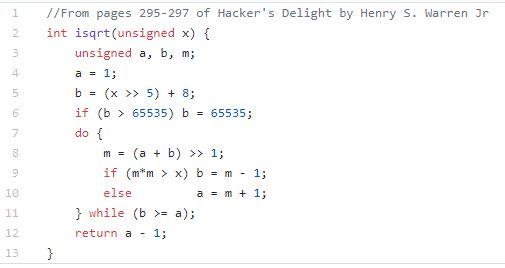
\includegraphics[width=\linewidth]{isqrt.jpg} 
\newpage
\noindent\textbf{Interview Question: Binary Search}\\
\indent Given an already sorted ArrayList of integers write a function in Java that finds the value $t$ from $n$ keys via binary search. Return $-1$ if $t$ is not in the list otherwise return the index.\\
\end{document}